\documentclass[12pt]{article}
\usepackage[utf8]{inputenc}
\usepackage[spanish]{babel}
\usepackage{newtxtext,newtxmath} % Times New Roman
\usepackage{setspace}
\setstretch{1.5}
\usepackage[letterpaper, left=3cm, right=2.5cm, top=2.5cm, bottom=2.5cm]{geometry} 
\usepackage{pdfpages} % Paquete para incluir PDFs

\begin{document}
	
	% Importar TODO el PDF
	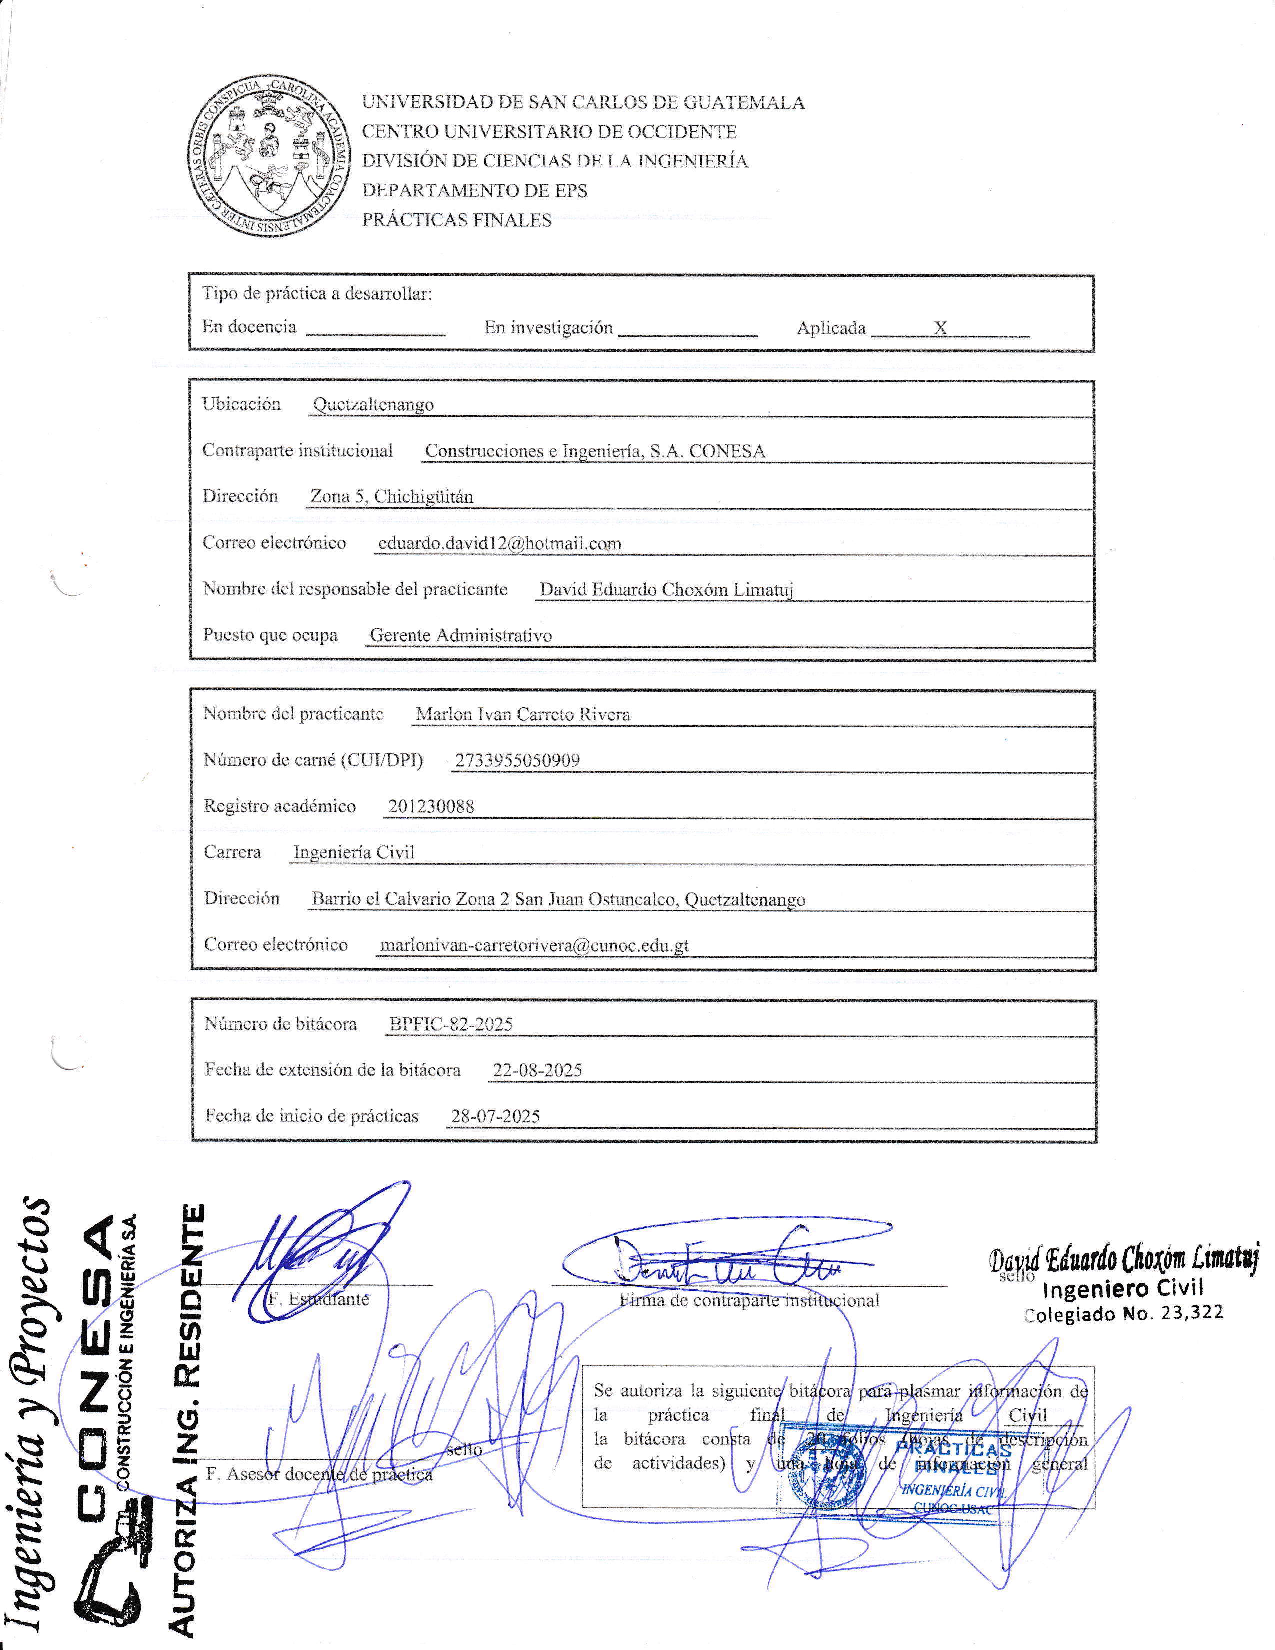
\includepdf[pages=-]{bitacorafolios}
	
	% Importar solo la primera página
	%\includepdf[pages=1]{archivo.pdf}
	
	% Importar un rango de páginas (ejemplo: 2 a 5)
%	\includepdf[pages=2-5]{archivo.pdf}
	
	% Importar páginas específicas (ejemplo: 1 y 3)
%	\includepdf[pages={1,3}]{archivo.pdf}
	
	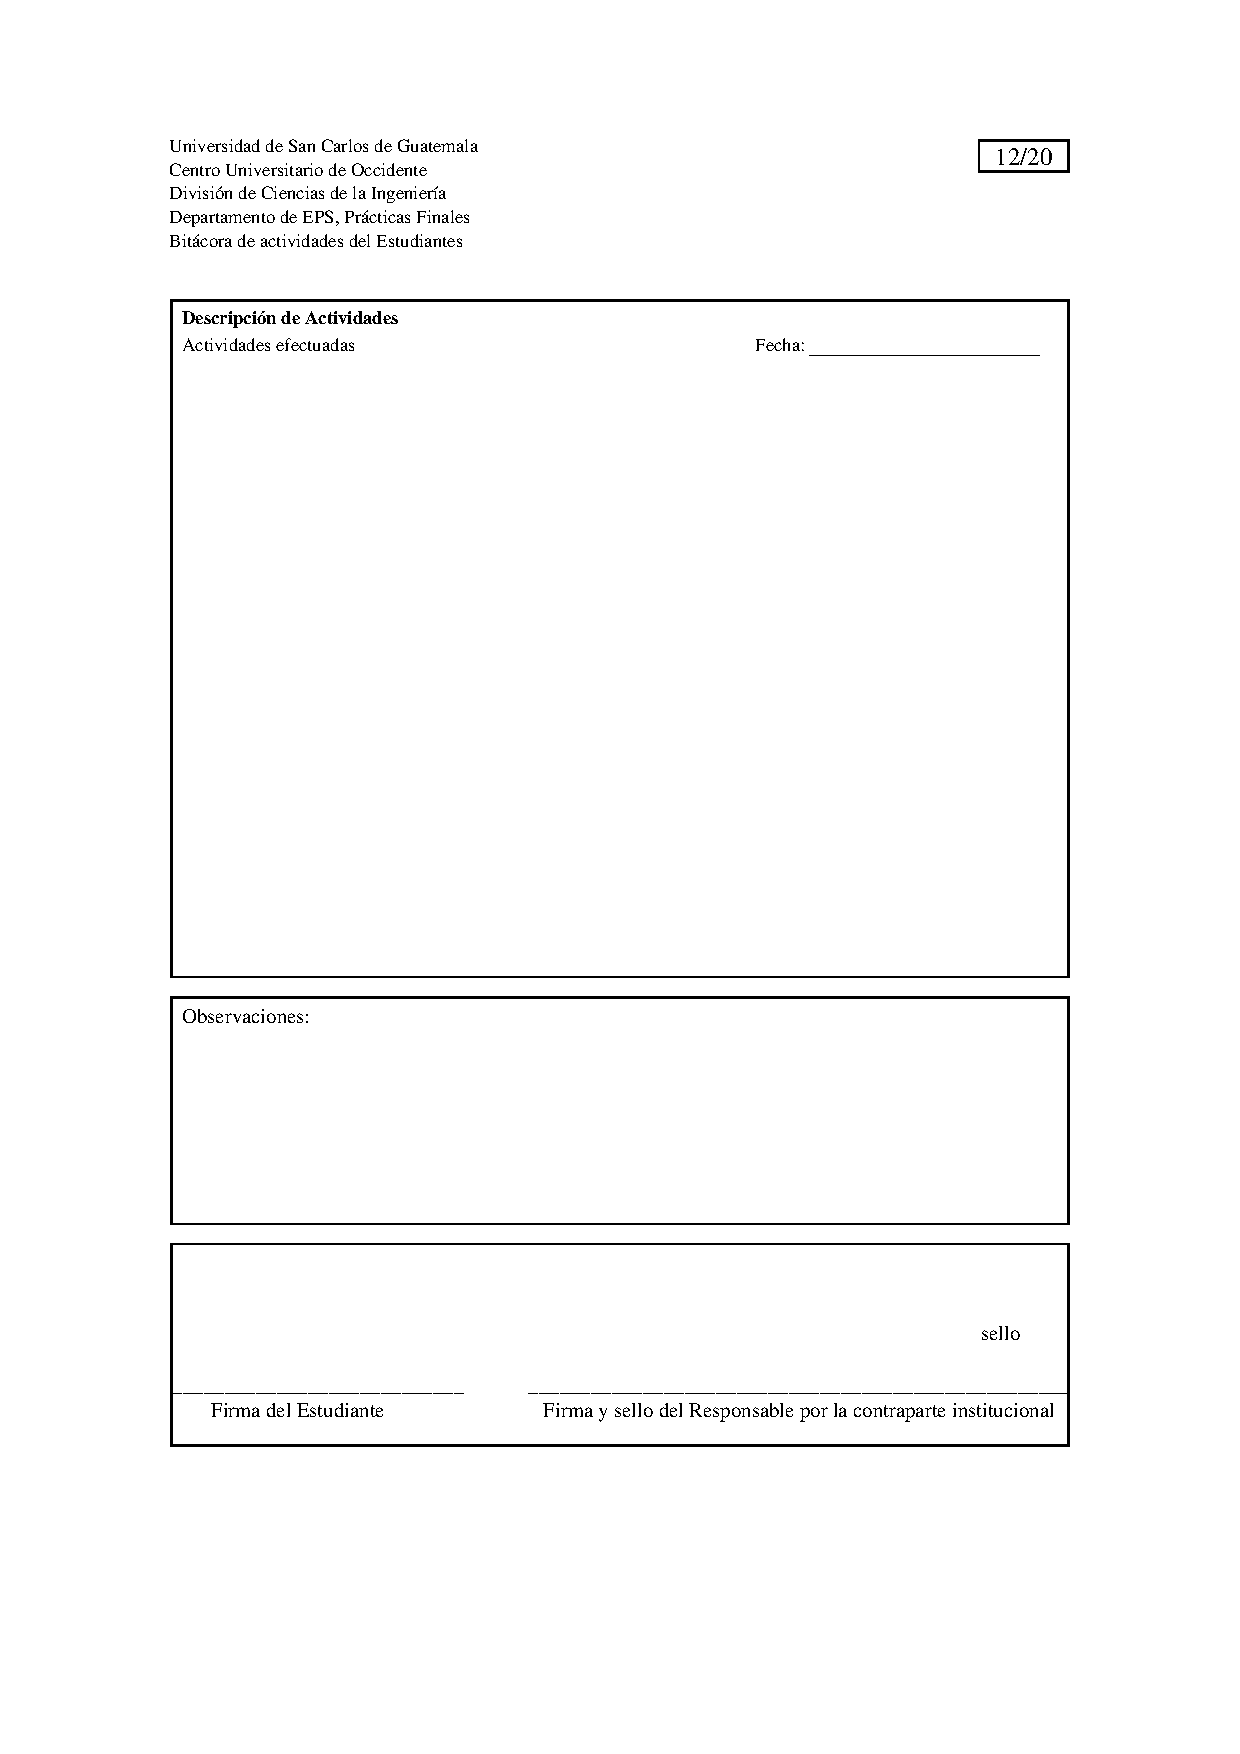
\includepdf[pages=-]{folios12a20}
	
\end{document}
